\chapter{THEORETICAL FRAMEWORK}
\normalsize{In this chapter, the basics of fusion such as nuclear physics and magnetic confinement are explained. In addition to that, the construction and the different systems of the W7-X are also explained to give an overview on the device and its auxiliary components. Heat transfer theory as well as solid mechanics including plasticity and fatigue constitute the basis of the work and the complex equations of these theories solved using Finite Element Analysis. These theories are necessary for the completion of this work and are therefore reminded in this chapter.}
\section{GENERAL THEORY OF FUSION REACTORS}
\normalsize{The principle of a nuclear fusion power plant is to make the energy released by the fusion of light atomic nuclei usable. Nuclear fusion which represent the fusing of atomic nuclei together is only achievable if they come close enough to surpass the electrostatic repulsion forces and have the strong nuclear force fuse the nucleons together. Due to electrostatic repulsion forces also called Coulomb barrier, the nuclei repulse each other thus preventing the reaching of the necessary distance (because the strong nuclear force has a very limited range, ~$10^{-15}$m) \cite{diekmann_energie:_2014}\cite{Freidberg_2007} for fusion. Furthermore, the repulsion forces increase with the number of protons in the nucleus or its size. The energy required to fuse two nuclei become subsequently greater.}
\\
\begin{figure}[h!] 
    \centering
    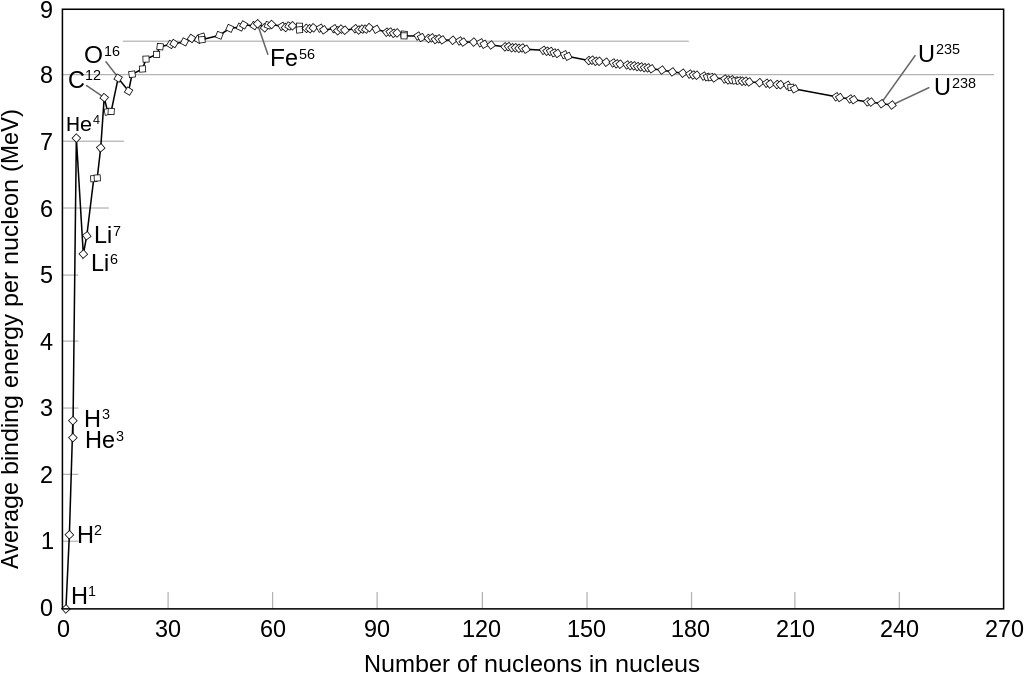
\includegraphics[width=.7\textwidth]{figures/fig_1.png}
    \caption{\it Nuclear binding energy vs. mass number.}
    \label{fig:fig_2_1}
\end{figure}
\\
\normalsize{\indent The different nuclear reactions for transforming hydrogen into helium are \cite{diekmann_energie:_2014}:}
\begin{equation}
    \ce{^1_1H + ^1_0n -> ^2_1H + 2.22 MeV\footnote{Automatically generated footnote markers work fine!}}
\end{equation}
\begin{equation}
    \ce{^2_1H + ^1_1p -> ^3_2He + 5.49 MeV}
\end{equation}
\normalsize{\indent or}
\begin{equation}
    \ce{^2_1H + ^2_1H -> ^3_2He + ^1_0n + 3.27 MeV}
\end{equation}
\begin{equation}
    \ce{^2_1H + ^2_1H -> ^3_1He + ^1_1p + 4.03 MeV}
\end{equation}
\begin{equation}
    \ce{^2_1H + ^3_1H -> ^4_2He + ^1_0n + 17.58 MeV}
\end{equation}
\\
\normalsize{\indent On Figure \ref{fig:fig_2_2}, the cross section for various reactions are graphed in function of the ion temperature. The cross section represents the area on which it is possible for nuclei to collide and subsequently fuse together. The higher the cross section, the higher the nuclei are likely to collide with each other. For lower ion temperatures, the Deuterium-Tritium reaction has the biggest cross section. The easiest way to initiate fusion is by the Deuterium–Tritium reaction, which releases $17.6 MeV$, $14.1 MeV$ in the neutron and $3.5 MeV$ in the alpha particle. \cite{Freidberg_2007}}
\\
\begin{figure}[h!]
    \centering
    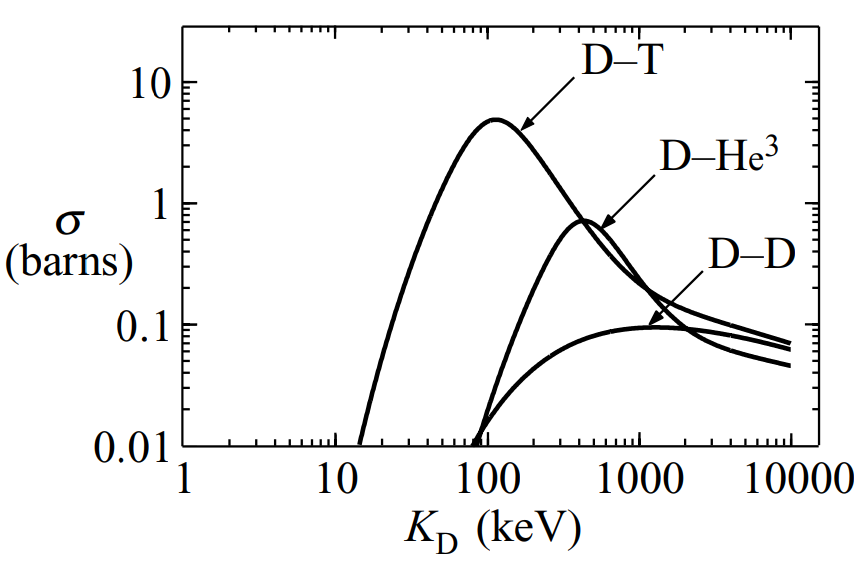
\includegraphics[width=.62\textwidth]{figures/crosssection.png}
    \caption{\it Fusion cross sections for various fusion reactions (D-T, D-$He^3$ and D-D) versus ion temperature. \cite{Freidberg_2007}}
    \label{fig:fig_2_2}
\end{figure}
\\
\normalsize{\indent When the cross section is known, is it possible to calculate the reaction rate for the main fusion reactions. The reaction rate is noted $\innerp{\sigma}{\nu}$. These results are illustrated in Figure \ref{fig:fig_2_3} as curves of $\innerp{\sigma}{\nu}$ vs. ion temperature $T$. It is possible to observe that the peak value of the reation rate is $9 \times 10^{-22} m^{3}s^{-1}$ at $70keV$ for the D-T fuel mix.}
\\
\begin{figure}[h!]
    \centering
    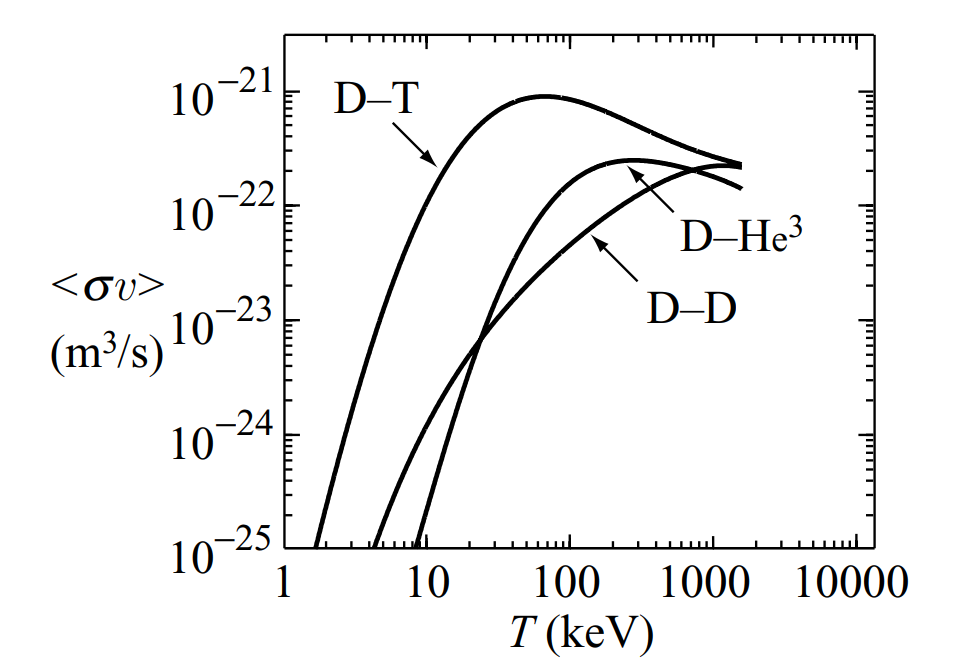
\includegraphics[width=.67\textwidth]{figures/reactionrate.png}
    \caption{\it Velocity averaged cross section $\innerp{\sigma}{\nu}$ for various fusion reactions (D-T, D-$He^3$ and D-D) versus ion temperature. \cite{Freidberg_2007}}
    \label{fig:fig_2_3}
\end{figure}
\\
\normalsize{\indent }
\\
\normalsize{\indent As said previously, the energies to achieve nuclear fusion are important. One solution to this problem is to give the correct amount of kinetic energy to the nuclei in order for them to overcome the Coulomb barrier. This kinetic energy is measured in Electron-Volts and is obtained by heating the fuel to high temperatures. The temperature thus reaches ~100M to 200M°C \cite{diekmann_energie:_2014}, which is hotter than the sun’s core. At those temperatures, the fuel becomes a plasma, which is often considered as the fourth state of matter. Plasma is also called the highest state of aggregation of a substance designated. In this aggregate state, the internal energy is far higher than the binding energy between the electrons and the nuclei. This means that the electrons can move freely. Plasma differs greatly in its properties from normal gases.}
\\
\break
\normalsize{\indent The important temperature of the plasma forces various measures to be taken to ensure that the Materials built into the fusion reactor near the plasma provide maintained thermal insulation and compensate for the resulting expansion pressure. A solution to this problem is the exploiting of the Lorenz force affecting the charged particles of the plasma. The idea is, at least for magnetic confinement, to trap the plasma inside a magnetic cage. This will help levitating the plasma and control its shape and position to avoid touching any \acrshort{PFCs}. The distance between the plasma and the \acrshort{PFCs} is crucial since contact could generate plasma turbulence or contaminate the plasma with impurities, reducing the quality of it. Different systems where developed to build such a confinement. }
\\
\break
\normalsize{\indent There are two different type of magnetic confinement concepts that are widely know and developed, the Tokamak and the Stellarator. These two magnetic confinement devices are both based on a toroidal geometry, the difference between the two of them being the way the plasma is confined. In a Tokamak machine, the plasma is confined using planar toroidal magnetic coils. Those coils help create the toroidal magnetic field component of the confinement. Although this seems like a good confinement, other problems still need to be addresses such as the effect of particle drift. This drift is due to  pressure gradients and inhomogeneities in the magnetic field inside the plasma and leads to a drift of the particles towards the outer diameter of the Tokamak. This complex particle transport phenomenon can be mitigated by introducing a poloidal component to the magnetic field, causing a rotation of the plasma around its toroidal axis. To achieve this magnetic field, Tokamaks use a solenoid coil placed at the center of the torus. This solenoid coil acts as a primary transformer coil, a time-varying electric current generate a varying magnetic field which itself induce an electric current inside the plasma. The resulting movement of charges inside the plasma generate a poloidal magnetic field, the plasma is then generating its own magnetic field. This electric current can also be used to heat up the plasma, it is called ohmic heating.}
\break
\begin{figure}[h!]
    \centering
    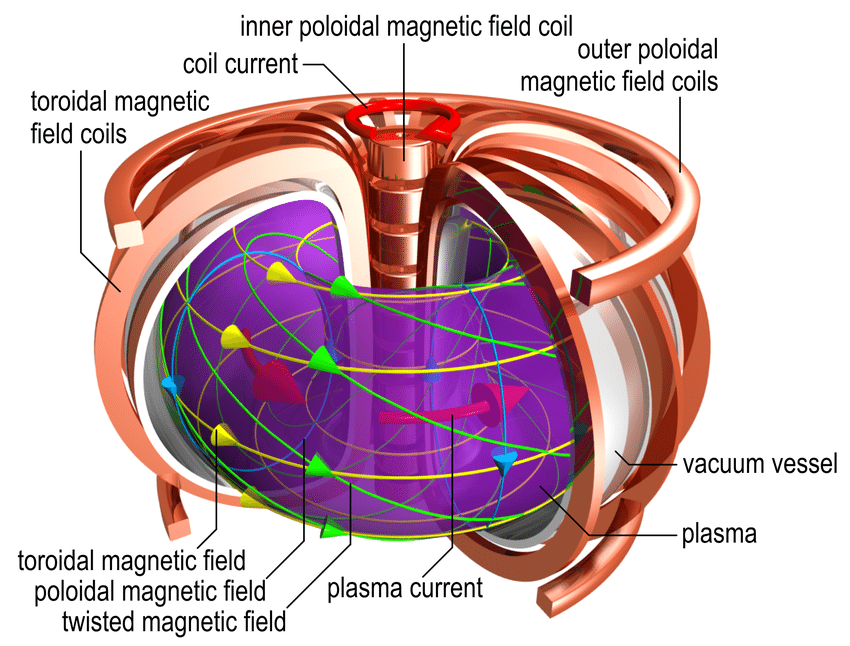
\includegraphics[width=.6\textwidth]{figures/fig_2.png}
    \caption{\it Schematics of a Tokamak confinement, courtesy of C. Brandt}
\end{figure}
\\
\break
\normalsize{\indent While this solution is good, there are problems with it. The main issue is the inherently transient process. The poloidal component of the magnetic field can only be generated as long as the current in the solenoid coil varies. This means that the reactor can only run in pulses and steady-state isn’t currently achievable.}
\\
\break
\normalsize{\indent Another solution for generating the poloidal magnetic field is to twirl the plasma in such a shape, that the drift phenomenon disappears. This solution is the Stellarator. The Stellarator was first introduced by Lyman Spitzer in the 1950s. This technology was put aside because of technical difficulties and because the Tokamaks presented better performances. The Stellarators use a complex set of magnets allowing to generate a precise magnetic field allowing the plasma to not experience significant drift. Contrary to Tokamaks, Stellerators plasmas don’t have a plasma current. This solution also helps with confinement, as the magnetic field can be adjusted to accommodate for the strict equilibrium conditions. The absence of plasma current also means that Stellarators can be operated in steady-state since no current induction is needed, thus being more suitable for power plants. Although allowing improved plasma confinement, Stellarators are plagued by complex geometries that are often too complex to be feasible.}
\begin{figure}[h!]
    \centering
    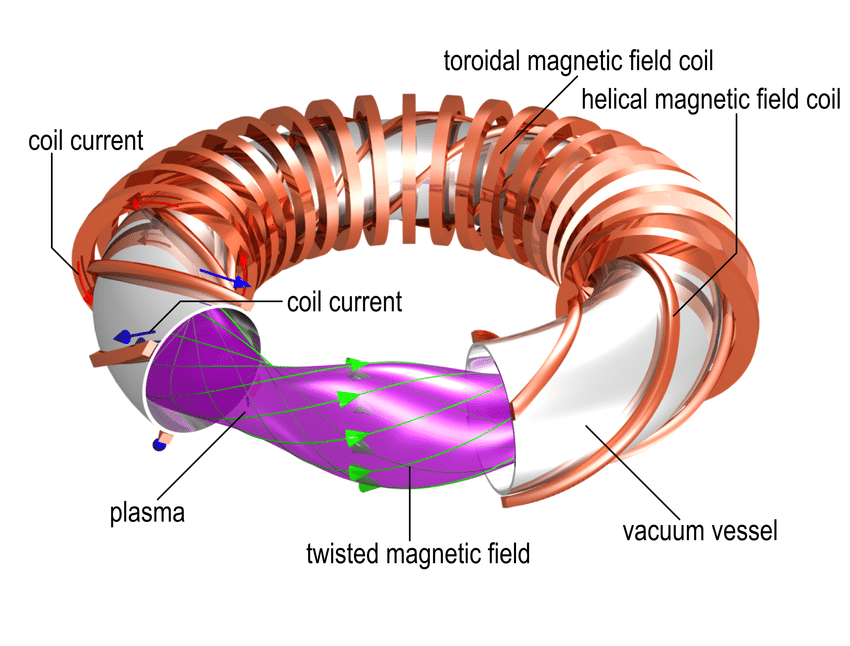
\includegraphics[width=.6\textwidth]{figures/fig_3.png}
    \caption{\it Schematics of a Stellarator confinement, courtesy of C. Brandt}
\end{figure}
\\
\normalsize{\indent The goal of those magnetic confinement fusion reactors concepts is to propose a new way of producing atomic energy while avoiding the drawbacks of traditional fission reactors (ie. Management of radiation, production of highly radioactive long half-life elements, limited fuel supply…). Although fusion energy is attractive, many problems still need to be addresses such as tritium breeding issues or neutron transport and interaction with the structure.}
\section{W7-X SYSTEMS}
\normalsize{he Wendelstein 7-X (W7-X) is a stellarator nuclear fusion experiment with a significant history that underscores its importance in fusion research. The idea for W7-X was born in the late 1980s and early 1990s, aimed at testing the viability of stellarator design for sustained fusion reactions. This project built upon the success of its predecessor, Wendelstein 7-AS.}
\\
\break
\normalsize{\indent In 1996, the German government approved the construction of W7-X, with substantial funding from the European Union and international partners. Construction began in 1997 at the Max Planck Institute for Plasma Physics (IPP) in Greifswald, Germany. This phase involved assembling complex superconducting magnetic coils and a highly precise vacuum vessel, presenting numerous technical challenges that required innovative solutions.}
\\
\break
\normalsize{\indent By 2014, the assembly of W7-X was completed, marking a major milestone. The machine produced its first plasma on December 10, 2015, demonstrating the functionality of its design and construction. Following this achievement, W7-X entered its experimental phase. Initial experiments focused on achieving and maintaining stable plasma conditions, testing heating methods, and studying plasma behavior.}
\\
\break
\normalsize{\indent Over the subsequent years, W7-X achieved several key milestones, including sustained plasma discharges lasting up to 100 seconds and significant advancements in plasma heating and density. These experiments provided valuable insights into plasma confinement and stability, moving closer to the goal of long-pulse operations lasting up to 30 minutes. This capability is critical for the development of future fusion power plants, as it demonstrates the potential of stellarators for continuous operation.}
\\
\break
\normalsize{\indent Research continues to optimize plasma performance, improve heating and control techniques, and deepen the understanding of stellarator physics. The Wendelstein 7-X remains a cornerstone of global fusion research, contributing valuable data and insights that support the broader goal of developing practical and sustainable fusion energy.}
\\
\section{HEAT TRANSFER}
\normalsize{In this section, the fundamental principles and governing equations and each heat transfer mode are explored. The TZM-reflector tile is a highly constrained mechanical part that of the \acrshort{HS}. This part will be exposed to plasma radiation as well as the \acrshort{ECRH} beam. The heat transfer in this system is complex and need a good understanding of the theory to model it as good as possible.}
\\
\normalsize{\indent The heat loads on the \acrshort{ECRH} reflector tile are specified further in the thesis but the theory first needs to be explained, at least what will be needed for this task.}
\\
\subsection{General problem of heat exchange}
\normalsize{Heat exchange happens all the time and everywhere in nature, from the sun's radiative power to the heat transfer on the surface of the skin. Historically, heat was considered as some sort of {\it flow} that would flow from one hot object to another colder object \cites{ahtt6e}. The idea of an invisible fluid flowing from a body to another called {\it Caloric} was first considered to explain this heat transport. While the caloric theory of heat exchange is acceptable to consider such a concept for explaining heat transport, there are more modern approaches to heat exchange that will be discussed later \cites{ahtt6e}. The general problem of heat transfer involves understanding how thermal energy is transported from one place to another. The modern aproach to heat transfer is the {\it kinetic} theory. Heat is defined to be the average Velocity of the particules within an system. This approach helps to understanding what heat is physically \cites{cengel2004heat}. Heat exchange can be seen in many different situations and takes place in every medium and different modes. Leaving a hot house during winter with a door open and having the hot air making its way out, hummingbirds using a counterflow heat exchanger in their feet to regulate their body temperatures \cites{UDVARDY_1983} or inadvertedly touching a hot pan are all examples of heat exchange between mediums and objects \cites{ahtt6e}. It respects some rules such as the flow direction, from hot to cold.}
\\
\break
\normalsize{\indent Not only in nature but also in industry, heat is heavily used for/or is a product of chemical processes. Steam boilers convert chemical energy into heat to generate steam and then generate elctricity, this is also true for nuclear power plants, using the heat generated by fission reactions to generate steam. Heat is generated in combustion engines and needs to be evacuated meanwhile in fridges, heat in pumped to decrease the temperature in a chamber. Those devices all use some sort of heat transfer in order to work properly. Heat exchange is also present throughout of fusion devices at many different levels such as inside the plasma as well as the first wall components and the pumping system. Correctly modelling heat exchange as well as understanding the physical phenomena behind the transfer of heat in thermal machines.}
\\
\break
\normalsize{\indent Thermodynamics is a theory about the dynamics and conversion of different energy forms heavily developed during the 19th century. It provides a very good framework in which it is possible to built a theory of heat exchange \cites{ahtt6e}. It is possible to derive the equation of heat transfer from the laws of thermodynamics. The first law of thermodynamics for a closed system, as taught in engineering programs, takes the following form:}

\subsection{Heat conduction}
\normalsize{Conduction is the transfer of energy from the more energetic particles of a substance to the adjacent less energetic ones as a result of interactions between the particles \cites{cengel2004heat}. Conduction can take place in solids, liquids, or gases. In fluids, conduction is due to the collision and diffusion of the molecules during their random motion. In solids, conduction is due to the combination of vibration of the molecules in a lattice and the energy transport by free electrons.}
\\
\break
\normalsize{\indent Lets consider steaty-state heat conduction through a plane wall of thickness $L  = \Delta x$ and area $A$. The difference of temperature or {\it gradient} is measured and is written $\Delta T = T_2 - T_1$. Experience has shown that the rate of heat transfer $\dot{Q}_{cond}$ through the wall would double when the temperature gradient across the wall {\it or} when when the area $A$ normal to the direction of heat transfer doubles. The rate of heat transfer would be halved when the thickness $L$ doubled. Qualitavively, it is possible to conclude that the rate of heat conduction through a plane wall is proportional to the temperature gradient across the layers and the heat transfer area, but is inverssely proportional to the thickness of the layer. The relation between the quantities is :}
\\
\begin{equation}
    (Rate \ of \ heat \ conduction) \propto \frac{(Area)(Temperature \ gradient)}{Thickness}
    % \tagaddtext{[\si{\watt}]}
    \label{eqn:CondEq}
\end{equation}
\\
\normalsize{\indent Analytically, the mathematical law describing the conduction of heat is {\bfseries Fourier's law of heat conduction}. The coefficient $k$ is the thermal conductivitiy, which is the abilitiy of a certain material to conduct heat. It is possible to write this law using quantities and the equation is :}
\\
\begin{equation}
    \dot{Q}_{cond} = -kA\frac{T_2 - T_1}{\Delta x} = -kA\frac{\Delta T}{\Delta x}
    \tagaddtext{[\si{\watt}]}
    % \tagaddtext{[\si{\watt}]}
    \label{eqn:CondEqInt}
\end{equation}
\\
\normalsize{When $\Delta x \rightarrow 0$,  the one-dimensionnal differential form of the equation is written:}
\\
\begin{equation}
    \dot{Q}_{cond} = -kA\frac{dT}{dx}
    \tagaddtext{[\si{\watt}]}
    \label{eqn:CondEq}
\end{equation}
\\
\normalsize{\indent On the left hand side of the heat conduction equation \refeq{eqn:CondEq} $\dot{Q}_{cond}$ decribes the time derivative or temporal rate of change of the heat flux flowing though a surface. On the the right hand side of the equation, k is the thermal conductivity. Usually, the thermal conductivity is a function of the temperature itself making this differential equation nonlinear. }
\\
\subsection{Convective heat transfer}
\normalsize{It was mentionned earlier that there are three basic mechanisms of heat transfer: conduction, convection, and radiation. Conduction and convection are similar in that both mechanisms require the presence of a material medium. But they are different in that convection requires the presence of fluid motion. Heat transfer through a solid is always by conduction, since the molecules of a solid remain at relatively fixed positions. Heat transfer through a liquid or
gas, however, can be by conduction or convection, depending on the presence of any bulk fluid motion. Heat transfer through a fluid is by convection in the presence of bulk fluid motion and by conduction in the absence of it.}
\subsection{Thermal radiation}

\section{SOLID MECHANICS}

\section{FINITE ELEMENT METHOD}

